\documentclass{article}

% Language setting
% Replace `english' with e.g. `spanish' to change the document language
\usepackage[T2A]{fontenc}
\usepackage[english, russian]{babel}

% Set page size and margins
% Replace `letterpaper' with `a4paper' for UK/EU standard size
\usepackage[letterpaper,top=2cm,bottom=2cm,left=3cm,right=3cm,marginparwidth=1.75cm]{geometry}

% Useful packages
\usepackage{amsfonts,amsmath,amssymb,amsthm}
\usepackage{breqn}
\usepackage{graphicx}
\graphicspath{ {./images/} }
\usepackage[colorlinks=true, allcolors=blue, backref=false]{hyperref}
\usepackage[T2A]{fontenc}

\makeatletter
\newenvironment{sqcases}{%
  \matrix@check\sqcases\env@sqcases
}{%
  \endarray\right.%
}
\def\env@sqcases{%
  \let\@ifnextchar\new@ifnextchar
  \left\lbrack
  \def\arraystretch{1.2}%
  \array{@{}l@{\quad}l@{}}%
}
\makeatother


\title{Рассмотрение возможных стратегий для получения оптимального распределения вероятностей в задаче о многоруких бандитах}
\author{Михаил Давыдов}

\begin{document}
\maketitle

\section{Постановка задачи и метрики}

Если параметры распределений известны для нас (но не для алгоритма) в ходе тестирования, то для измерения результата можно использовать 3 метрики. Каждая из наград считается по каждому шагу и усредняется по нескольким сгенерированным различным независимым задачам о многоруких бандитах.
\begin{enumerate}
    \item Ожидаемый портфель $\text{Portf}_t = m_{p_t} - \lambda \sigma_{p_t}^2$. Метрика аналогична награде для обычной задачи о многоруких бандитах. В качестве альтернативы можно использовать сожаление $\text{Regret}_t = \underset{P}{\max} \left( m_p - \lambda \sigma_p^2 \right) - \text{Portf}_t$
    \item Так как мы хотим, чтобы вероятности сошлись к оптимальным как можно быстрее, то можно использовать усредненный по шагам портфель $\overline{\text{Portf}_t} \frac{\sum_{k=1}^t m_{p^k} - \lambda \sigma_{p^k}^2}{t}$ или усредненное сожаление $\overline{\text{Regret}_t} = \underset{P}{\max} \left( m_p - \lambda \sigma_p^2 \right) - \overline{\text{Portf}_t}$.
    \item Пусть вектор вероятностей, при котором достигается макисмальное значение $m_p - \lambda \sigma_p^2$, равен $P = (p^1, ..., p^n)$. Зная $m_i$ и $\sigma_i^2$, его можно получить с помощью метода градиентного подъема (формулой воспользоваться не получится, так как вероятности в нашей задаче неотрицательны). Пусть также полученный вектор вероятностей в задаче о многоруких бандитах равен $B = (b_1, ..., b_n)$. Тогда метрика равна $$\delta = 1 - \frac{1}{2}\sum_{i=1}^n |b_i - p_i|$$
    Заметим, что в обычной задаче о многоруких бандитах $P = (0, ..., 1, 0, ..., 0)$, и новая метрика равна $1 - \frac{1}{2}\left( (1 - b_k) + \sum_{i = 1, i \neq k}^n b_i \right) = 1 - (1 - b_k) = b_k$, то есть совпадает с процентом оптимальных действий, а это есть вторая метрика в обычной задаче о многоруких бандитах. Так как $\delta \in [\underset{i}{\min} (p_i), 1]$, то можно также ввести ``растянутую'' метрику $\hat{\delta} = (\delta - \underset{i}{\min}(p_i) ) \cdot \frac{1}{1 - \underset{i}{\min}(p_i)} \in [0,1]$. Аналогично, можно считать ``сожаление'' и усредненное сожаление.
\end{enumerate}

\section{Подсчет матожидания и дисперсии}

Пусть $a$-ый рычаг на $t$-ом шаге был выбран всего $N_t(a)$ раз. Обозначим $R_i(a) = R_i \cdot \mathbb{I}(A_i = a)$. Будем приближать матожидание и дисперсию с помощью выборочного матожидания и выборочной дисперсии:
\begin{itemize}
    \item $Q_t(a) = \frac{\sum_{i=1}^{t-1} R_i(a)}{N_t(a)}$ -- выборочное матожидание -- так же, как и для обычной задачи о многоруких бандитах. Если $N_t(a) = 0$ или $t=1$, то $Q_t(a)$ = 0
    \item $S_t(a) = \frac{1}{N_t(a) - 1}\sum_{i=1}^{t-1}(R_i(a) - Q_t(a))^2 = \frac{N_t(a)}{N_t(a) - 1}(\overline{R_t^2(a)} - Q_t(a)^2)$ -- выборочная дисперсия, где $\overline{R_t^2(a)} = \frac{\sum_{i=1}^{t-1} R_i^2(a)}{N_t(a)}$. Если $N_t(a) \leq 1$, будем считать, что $S_t(a) = 0$.
\end{itemize}
Заметим, что $\mathbb{E}\,Q_t(a) = m_a$, $\mathbb{E}\,S_t(a) = \sigma_a^2$ (за исключением холодного старта, то есть случая $N_t(a) \leq 1$), и такие приближения корректны. Кроме того:
\begin{itemize}
    \item Для невыбранных на $t$-ом шаге рычагов обновления выборочного матожидания и дисперсии не происходит.
    \item $Q_{t+1}(A_t) = Q_t(A_t) + \frac{1}{N_{t}(A_t) + 1}(R_t - Q_t(A_t))$, поэтому обновление выборочного матожидания происходит за $O(1)$.
    \item Для дисперсии:
    \begin{dmath}
        S_{t+1}(A_t) = \frac{N_t(A_t) + 1}{N_t(A_t)} \left( \overline{R_{t+1}^2(A_t)} - Q_{t+1}^2(A_t)\right) = \frac{N_t(A_t) + 1}{N_t(a)} \left( \overline{R_t^2(A_t)} \frac{N_t(A_t)}{N_t(A_t) + 1} + \frac{R_t^2}{N_t(A_t) + 1} - \overline{R_t^2(A_t)} \frac{N_t(A_t)}{(N_t(A_t) + 1)^2} - 2Q_t(A_t)R_t\frac{N_t(A_t)}{(N_t(A_t) + 1)^2} - \frac{R_t^2}{(N_t(A_t) + 1)^2} \right) = \frac{N_t(A_t) \overline{R_t^2(A_t)} - 2Q_t(A_t)R_t + R_t^2}{N_t(A_t) + 1}\label{eq:1}
    \end{dmath}
    Аналогично $Q_t(A_t)$,  $\overline{R_{t+1}^2(A_t)} = \overline{R_t^2(A_t)} + \frac{1}{N_{t}(A_t) + 1}(R_t - \overline{R_t^2(A_t)})$ -- считается за $O(1)$. Тогда и $S_{t+1}(A_t)$ можно по формуле (\ref{eq:1}) пересчитать за $O(1)$.
\end{itemize}

\section{Стратегии}

В этой секции мы рассмотрим подходы для нахождения оптимального вектора вероятностей. Будут представлены аналоги greedy, $\epsilon$-greedy, Optimistic стратегий, UCB, Gradient bandits а также сэмплирование Томпсона. Далее всегда будем считать, что в первый ход рычаг выбирается случайно, то есть $P_1 = \left( \frac{1}{n}, ..., \frac{1}{n} \right)$.

\subsection{Greedy стратегии}

\subsubsection{Итеративные greedy стратегии}

В отличие от обычной задачи о многоруких бандитах, в новой версии для greedy стратегий вектор вероятностей выбора $P_t$ может быть не равен вектору $(0, ..., 1, 0, ..., 0)$. Каждый шаг будем менять вероятность выбора каждого рычага в соответствии с новой полученной наградой. ``Жадность'' будет выражаться в несколько другом смысле. Опишем сначала процесс изменения вероятностей для итеративных greedy-стратегий. Под итеративными стратегиями понимаются стратегии, которые при заданных матожиданиях и дисперсиях сходятся к оптимальному вектору вероятностей за $k > 1$ проходов какого-то кода, но на каждом шаге производящих только один проход этого кода.

Пусть на $t$-ом шаге вектор вероятностей равен $P_t = (p_t^1,...,p_t^n)$. Будем на каждом шаге изменять вероятности так, чтобы максимально увеличить $V = Q_{t,p} - \lambda S_{t,p}^2$, где $Q_{t,p} = \sum_{i=1}^n p_t^i Q_t(i)$, $S_{t,p}^2 = \sum_{i=1}^n (p_t^i)^2 S_t(i)^2$. Можно рассмотреть 2 подхода:
\begin{enumerate}
    \item\label{sec:1} Каждый ход будем увеличивать одну из вероятностей $p_i$ на $\Delta p \geq 0$, а другую вероятность $p_j$ -- уменьшать на $\Delta p$. Сумма вероятностей не изменилась. Будем искать такие $i, \, j, \, \Delta p$, что $p_i^{new} \leq 1, p_j^{new} \geq 0$ и увеличение $V \; (:= \Delta V)$ максимально. Заметим, что $p_i + \Delta p \leq 1 \Leftrightarrow \Delta p \leq 1 - p_i$, $\: p_j - \Delta p \geq 0 \Leftrightarrow \Delta p \leq p_j$ и $1 - p_j \geq p_i \Leftrightarrow p_i + p_j \leq 1$, поэтому условие $p_i^{new} \leq 1$ избыточно. После изменения соответствующих вероятностей получим:
    \begin{dmath}
        \Delta V =\left[ (p_i + \Delta p) Q_t(i) + (p_j - \Delta p) Q_t(j) - \lambda (p_i + \Delta p)^2 S_t^2(i) - \lambda (p_j - \Delta p) S_t^2(j) \right] - \left[  p_i Q_t(i) + p_j Q_t(j) - \lambda p_i^2 S_t^2(i) - \lambda p_j^2 S_t^2(j) \right] = \Delta p (Q_t(i) - Q_t(j)) - 2 \lambda \Delta p (p_i S_t^2(i) - p_j S_t^2(j)) - \lambda (\Delta p)^2 \left[ S_t^2(i) + S_t^2(j) \right] = \Delta p \left( [Q_t(i) - 2 \lambda p_i S_t^2(i)] - [Q_t(j) - 2 \lambda p_j S_t^2(j)]\right) - \lambda (\Delta p)^2 \left[ S_t^2(i) + S_t^2(j) \right] \overset{w_k := Q_t(k) - 2 \lambda p_k S_t^2(k)}{=} (w_i - w_j) \Delta p - \lambda \left[ S_t^2(i) + S_t^2(j) \right] (\Delta p)^2
        \label{eq:2}
    \end{dmath}
    Если $\lambda > 0$, $S_t^2(i) \neq 0 \lor S_t^2(j) \neq 0$, то получили квадратный многочлен с отрицательным главным коэффициентом. Этот многочлен достигает максимума в точке $\Delta p = \frac{w_i - w_j}{2 \lambda (S_t^2(i) + S_t^2(j))}$ и этот максимум равен $\frac{(w_i - w_j)^2}{4 \lambda \left[ S_t^2(i) + S_t^2(j) \right]}$. Заметим, что $w_i - w_j = - (w_j - w_i)$ и поэтому при перестановке $i$ и $j$ значение $\Delta p$ изменится на противоположное, поэтому $p_i + \Delta p$ и $p_j - \Delta p$ не изменятся, как и ограничения на них. Для удобства будем рассматривать только такие пары $(i,j)$, что $w_i - w_j \geq 0$. Так как отрезок $\left[0, \min \left(p_j, \frac{w_i - w_j}{2 \lambda \left[ S_t^2(i) + S_t^2(j) \right]} \right) \right]$ находится левее точки максимума, то при заданных ограничениях максимум $\Delta V$ достигается при $\Delta p = \min \left( p_j, \frac{w_i - w_j}{2 \lambda \left[ S_t^2(i) + S_t^2(j) \right]} \right)$. Посчитав $\Delta V$ для всех пар $(i,j)$ с $w_i - w_j > 0$, сможем найти оптимальные $i, \, j, \, \Delta V$.

    Если $\lambda = 0$, то задача сводится к обычной задаче о многоруких бандитах. Если же $S_t^2(i) = S_t^2(j) = 0$, то многочлен равен $\Delta p (Q_t(i) - Q_t(j)$. Опять, можно считать, что $Q_t(i) \geq Q_t(j)$, так как иначе знак $\Delta p$ меняется на противоположный, и максимальное значение $\Delta V$ не меняется. Тогда оптимальное $\Delta p = p_j$ и $\max \Delta V = (Q_t(i) - Q_t(j)) p_j$. Тот факт, что $S_t^2(i) = 0$, означает, что или количество нажатий на $i$-ый рычаг $ \leq 1$, или $i$-ый рычаг всегда выдаёт одно и то же значение (то есть рычаг безрисковый), или распределение $i$-го рычага дискретное, но все полученные до этого значения при нажатии на $i$-ый рычаг были одинаковыми. В случае, когда оба рычага безрисковые, и эти 2 рычага были выбраны для изменения вероятностей, $p_j^{new} = 0$, то есть безрисковый рычаг с меньшим значением больше не будет выбираться, как и в оптимальном векторе вероятностей. 

    Обратим внимание на проблему холодного старта: после первого шага, когда был выбран только один $i$-ый рычаг, может оказаться, что полученная награда $> 0$, в то время как выборочные дисперсии всех рычагов и выборочное матожидание всех других рычагов нулевое. В таком случае наибольшая разница $\Delta V$ будет достигаться при увеличении вероятности выбранного рычага на $\frac{1}{n}$ и уменьшении вероятности какого-то другого рычага $j$ до $p_j^{new} = 0$. То есть $j$-ый рычаг больше не будет выбран, хотя он может быть ``лучше'' $i$-го рычага. Если же полученная награда $< 0$, то тогда обнулится вероятность выбора $i$-го рычага, хотя нам могло просто не повезти с наградой. О том, как справляться с этой проблемой, мы поговорим позднее.

    Кроме того, алгоритм каждый шаг меняет всего 2 вероятности, что медленно, а сам шаг совершается за $O(n^2)$ (в то время как greedy-стратегия в оюычной задаче о многоруких бандитах -- за $O(n)$).
    \item В качестве альтернативы можно пытаться за один шаг менять сразу все вероятности. Одна из вероятностей будет изменяться в одну сторону, а остальные -- в другую. Отдельно будем рассматривать случаи с увеличением этой единственной вероятности и с ее уменьшением.
    
    Пусть на $t$-ом шаге $\phi_t$ рычагов с ненулевыми вероятностями выбора, то есть $|\{i: p_t^i \neq 0\}| = \phi_t$ и пусть $K_t := \{i: p_t^i \neq 0\}$. Будем каждый ход увеличивать одну из вероятностей $p_i$ на $\Delta p_{\uparrow}$, а все остальные ненулевые вероятности -- уменьшать на $\frac{\Delta p_{\uparrow}}{\phi_{t,i}}$, где $\phi_{t,i} := \phi_t - \mathbb{I}_{p_i \neq 0}$. Сумма вероятностей не изменилась. Будем искать такие $i, \, \Delta p_{\uparrow}$, что $\forall j \hookrightarrow 1 \geq p_j^{new} \geq 0$ и значение $\Delta V_{\uparrow}$ максимально. Если $\phi_{t,i} = 0$, то $p_i = 1$, и $\Delta p_{\uparrow} = \Delta V_{\uparrow} = 0$. Иначе после изменения соответствующих вероятностей получим:
    \begin{dmath}
        \Delta V_{\uparrow} = \Delta p_{\uparrow} \left(Q_t(i) - \frac{\sum_{\substack{j \in K_t \\ j \neq i}} Q_t(j)}{\phi_{t,i}} \right) - 2\lambda \Delta p_{\uparrow} \left( p_i S_t^2(i) - \frac{\sum_{\substack{j \in K_t \\ j \neq i}} p_j S_t^2(j)}{\phi_{t,i}} \right) - \lambda (\Delta p_{\uparrow})^2 \left( S_t^2(i) + \frac{\sum_{\substack{j \in K_t \\ j \neq i}} S_t^2(j)}{\phi_{t,i}^2} \right) = \Delta p_{\uparrow} \left( w_i - \frac{\sum_{\substack{j \in K_t \\ j \neq i}} w_j}{\phi_{t,i}} \right) - \lambda (\Delta p_{\uparrow})^2 \left( S_t^2(i) + \frac{\sum_{\substack{j \in K_t \\ j \neq i}} S_t^2(j)}{\phi_{t,i}^2} \right) = \Delta p_{\uparrow} \frac{\sum_{\substack{j \in K_t \\ j \neq i}} (w_i - w_j)}{\phi_{t,i}} - \lambda (\Delta p_{\uparrow})^2 \frac{\sum_{\substack{j \in K_t \\ j \neq i}} (\phi_{t,i} S_t^2(i) + S_t^2(j))}{\phi_{t,i}^2}
        \label{eq:3}
    \end{dmath}
    Если $\lambda \neq 0$ и $\exists j \in K_t \cup \{i\} \hookrightarrow S_t^2(j) \neq 0$, то получаем квадратный многочлен, максимум которого в точке
    $$\Delta p_{\uparrow} = \frac{\phi_{t,i} \sum_{\substack{j \in K_t \\ j \neq i}} (w_i - w_j)}{2\lambda \sum_{\substack{j \in K_t \\ j \neq i}} ( \phi_{t,i} S_t^2(i) + S_t^2(j) )}$$
    и в этой точке достигается значение
    $$ \Delta V_{\uparrow} = \frac{\left( \sum_{\substack{j \in K_t \\ j \neq i}} (w_i - w_j) \right)^2}{4\lambda \sum_{\substack{j \in K_t \\ j \neq i}} ( \phi_{t,i} S_t^2(i) + S_t^2(j) )}
    $$
    Здесь уже может быть $\Delta p_{\uparrow} < 0$. Если $\Delta p_{\uparrow} \geq 0$, то налагаются дополнительные ограничения $p_i^{new} \leq 1 \Leftrightarrow \Delta p_{\uparrow} \leq 1 - p_i$ и $\forall j \in K_t \setminus \{i\} \hookrightarrow p_j^{new} \geq 0 \Leftrightarrow \Delta p_{\uparrow} \leq \phi_{t,i} p_j$. Если же $\Delta p_{\uparrow} < 0$, то налагаются ограничения $p_i^{new} \geq 0 \Leftrightarrow \Delta p_{\uparrow} \geq -p_i$ и $\forall j \in K_t \setminus \{i\} \hookrightarrow p_j^{new} \leq 1 \Leftrightarrow \Delta p_{\uparrow} \geq \phi_{t,i} (p_j - 1)$. Итоговое $\Delta p_{\uparrow}$ берется как минимум (при $\Delta p_{\uparrow} \geq 0$) или как максимум (при $\Delta p_{\uparrow} < 0$) от аргмаксимума функции и ограничений.

     Если $\lambda = 0$, то задача сводится к обычной задаче о многоруких бандитах. Если же $\forall j \in K_t \cup \{i\} \hookrightarrow S_t^2(j) = 0$ (то есть безрисковые рычаги или $N_t(i) \leq 1$), то уравнение линейно или всегда равно 0 и достигает максимума в минимуме (если коээфициент $\geq 0$) или максимуме (если $\leq 0$) из ограничений.

     Аналогично, можно пытаться уменьшить одну вероятность $p_i$ на $\Delta p_{\downarrow}$, а все остальные, не равные 1 (пусть таких $\psi_{t,i}$) -- увеличить на $\frac{\Delta p_{\downarrow}}{\psi_{t,i}}$. Пусть $K_t = \{j: j \land p_j \neq 1 \}$. Проводя аналогичные вычисления, получим формулы:
     $$
     \Delta p_{\downarrow} = \frac{-\psi_{t,i} \sum_{\substack{j \in K_t \\ j \neq i}} (w_i - w_j)}{2\lambda \sum_{\substack{j \in K_t \\ j \neq i}} ( \psi_{t,i} S_t^2(i) + S_t^2(j) )}, \; \Delta V_{\downarrow} = \frac{\left( \sum_{\substack{j \in K_t \\ j \neq i}} (w_i - w_j) \right)^2}{4\lambda \sum_{\substack{j \in K_t \\ j \neq i}} ( \psi_{t,i} S_t^2(i) + S_t^2(j) )}
     $$
     На $\Delta p_{\downarrow}$ накладываются аналогичные ограничения, аналогично в случае, когда многочлен линейный. Аналогично вычисляется оптимальное $\Delta p$.

     Сравнивая все $\Delta V_{\uparrow}$ и $\Delta V_{\downarrow}$, найдем оптимальные $i, \, \Delta_p$ и тип измененния ($\uparrow$ или $\downarrow$).

     Нам нужно проверить 2 различных варианта для каждого рычага. Каждая проверка проходит за $O(n)$ (проверка на равенство 0 или 1, вычисление $\Delta_p$ и наложение не более $n$ ограничений), поэтому шаг алгоритма работает за $O(n^2)$. При этом, так как в этом методе мы изменяем сразу все вероятности, а не две, то он сходится быстрее, чем второй метод~\autoref{sec:1}. Однако этот алгоритм гораздо сильнее страдает от проблемы холодного старта: если после первого шага при нажатии $i$-го рычага мы получили награду, большую 0, то наибольшее изменение $\Delta V$ будет достигаться для тройки $(i, \uparrow, \frac{n-1}{n})$, и вся вероятность сконцентрируется в $p_i$. Если затем всегда будет $Q_t(i) - \lambda S_t^2(i) > 0$, что вполне реально, то алгоритм всегда будет нажимать на $i$-ый рычаг, в то время как могут быть рычаги с большим матожиданием или меньшей дисперсией, на которые никогда не нажмут.

\subsubsection{Градиентный подъем}
Теперь опишем метод градиентного подъема. На каждом шаге $t$ рассмотрим функцию $Q_{t,p} - \lambda S_{t,p}^2 = \sum_{i=1}^n p_i Q_t(i) - \lambda \left( \sum_{i=1}^n p_i^2 S_t^2(i)\right)$. Заметим, что множество
     $$
     Q =
        \begin{cases}
           0 \leq p_1 \leq 1 \\
            ... \\
            0 \leq p_{n} \leq 1 \\
            p_1 + ... + p_n = 1
        \end{cases}
        \label{eq:4}
     $$
     есть $n$-мерный симплекс, а, значит, $Q$ выпукло и замкнуто. Далее, $V$ вогнута на $\mathbb{R}^n$, так как
     $$
     \frac{\partial V}{\partial p_i} = Q_t(i) - 2\lambda p_i S_t^2(i), \;
     \frac{\partial^2 V}{\partial p_i^2} = -2\lambda S_t^2(i), \;
     \frac{\partial^2 V}{\partial p_j \partial p_i} = 0 \; (j \neq i)
     $$
    и гессиан $V$ равен
    $$
    -2\lambda
    \begin{pmatrix}
        S_t^2(1)        &          &        &                  \\
                        & S_t^2(2) &        & \text{\huge{0}}  \\
        \text{\huge{0}} &          & \ddots &                  \\
                        &          &        & S_t^2(n)
    \end{pmatrix}
    \preceq 0
    $$
    и, кроме того, $V$ имеет липшицев градиент с параметром $2\lambda \sqrt{\underset{i}{\max}(S_t^2(i))}$, так как 
    \begin{multline}
        \sqrt{\frac{\| \nabla V (p) - \nabla V (q) \|_2^2}{\| p - q \|_2^2}} = \sqrt{\frac{4\lambda^2 \sum_{i=1}^n S_t^2(i) (p_i - q_i)^2}{\sum_{i=1}^n (p_i - q_i)^2}} \leq \\ \leq \sqrt{\frac{4\lambda^2 \underset{i}{\max}(S_t^2(i)) \sum_{i=1}^n (p_i - q_i)^2}{\sum_{i=1}^n (p_i - q_i)^2}} = 2\lambda \sqrt{\underset{i}{\max}(S_t^2(i))}
    \end{multline}
    Тогда метод градиентного отображения для функции $V' = -V$ сойдется к глобальному минимуму на $Q$, а, значит, для функции $V$ этот метод сойдется к глобальному максимуму на $Q$ \cite{nesterov_convergence}. В качестве альтернативы градиентному методу можно использовать проекцию градиента на симплекс \cite{simplex_projection}, вычисление которого происходит за $O(n)$, или Cauchy-Simplex метод \cite{cauchy_simplex}, тоже сходящийся к глобальному максимуму и требующий на каждом шаге $O(1)$ вычислений (однако серьезный минус заключается в очень медленной скорости сходимости $\| x^T - x^*\| \leq \frac{\log n}{T}$).

    Базовый алгоритм будет состоять в следующем: на каждом шаге $t$ выбираем рычаг согласно вероятностям $P_t$, обновляем выборочные дисперсии и матожидания, после чего с помощью градиентного подъема находим глобальный максимум $P_{t+1} = (p_{t+1}^1, ..., p_{t+1}^n)$ на $Q$, после чего повторяем алгоритм для $P_{t+1}$. Если обозначить $u$-ое значение метода градиентного подъема в ходе проведения алгоритма на шаге $t$ за $P_t^u$, а оптимальный вектор вероятностей на шаге $t$ за $P_t^*$, то тогда каждый шаг алгоритма работает за не более чем $O(k_t^{\Delta})$, где $k_t^{\Delta} = \underset{P \in Q}{\max} \min \{u: \| P_t^u - P_t^* \| \leq \Delta\}$ для заданной погрешности $\Delta$, так что шаг алгоритма может работать очень долго.

    Кроме того, никуда не делась проблема холодного старта: аналогично второму алгоритму, после первого шага все вероятности, кроме одной $p_t^i$, могут занулиться, и далее при $Q_t(i) - S_t^2(i) > 0$ вектор вероятностей не изменится.

    Изложенный выше алгоритм чем-то похож на Generalized Policy Iteration: процессом градиентного подъема можно считать policy evaluation, а нажатием рычага согласно вероятностям -- policy improvement \cite{suttonbarto_policy_iteration}. Однако здесь evaluation происходит одновременно еще и по матожиданию с дисперсией, и эти процессы друг с другом конфликтуют, что приводит к медленному или даже неверному приближению к ответу.
\end{enumerate}

В заключение этого параграфа стоит заметить, что для обычной задачи о многоруком бандите все три алгоритма работают как обычные greedy-алгоритмы. Более того, все три алгоритма, как и стандартный greedy-алгоритм, страдают от проблемы холодного старта. Эти алгоритмы не единственны, для приближения вероятностей можно использовать метод Ньютона, метод штрафных функций, а также вместо одной или всех вероятностей пытаться за один ход изменять $k$ вероятностей, где $k = const$.

\subsubsection{Быстрый greedy алгоритм}
Есть алгоритм, находящий за $O(n \log n)$ распределение вероятностей, максимизирующее $Q_{t,p} - \lambda S_{t,p}^2$. Далее для удобства вместо $Q_{t,p}$ будем писать $m_p$ и вместо $S_{t,p}^2$ будем писать $\sigma_p^2$. Тогда:
\begin{enumerate}
    \item Пусть $i,j \in \{1, ..., n\}, \; i \neq j$. До этого мы рассматривали функцию $V(p_1, ..., p_n) = m_p - \lambda \sigma_p^2$. Рассмотрим функцию
    \begin{dmath}
        V(p_1, ..., p_n, \alpha) = p_1 m_1 + ... + (p_i + \alpha) m_i + ... + (p_j - \alpha) m_j + ... + p_n m_n - \lambda (p_1^2 \sigma_1^2 + ... + (p_i + \alpha)^2 \sigma_i^2 + ... + (p_j - \alpha)^2 \sigma_j^2 + ... + p_n^2 \sigma_n^2)
    \end{dmath}
    То есть $V(p_1, ..., p_n, \alpha) = V(p_1, ..., p_i + \alpha, ..., p_j - \alpha, ..., p_n)$. Возьмем точку $P^* \in Q$ (см. \ref{eq:4}), в которой достигается максимум $V$ на $Q$. Предположим, что $p_i^* \neq 1$ и $p_j^* \neq 0$. Тогда $\exists \delta > 0: \: \forall \alpha: \: 0 \leq \alpha < \delta \hookrightarrow P^*(\alpha) = (p_1^*, ..., p_i^* + \alpha, ..., p_j^* - \alpha, ..., p_n^*) \in Q$, и потому функция $V(p_1, ..., p_n, \alpha)$, определенная при $P \in Q, 0 \leq \alpha \leq \delta$, дифференцируема в точке $(P^*, 0)$ причем:
    \begin{dmath}
        \frac{\partial V(p_1, ..., p_n, \alpha)}{\partial \alpha}\bigg|_{P = P^*, \, \alpha = 0} = \left( (m_i - 2\lambda p_i^* \sigma_i^2 - \alpha \lambda \sigma_i^2) + (-m_j + 2\lambda p_j^* \sigma_j^2 - \alpha \lambda \sigma_j^2) \right) \bigg|_{\alpha = 0}  = (m_i - 2 \lambda p_i^* \sigma_i^2) - (m_j - 2 \lambda p_j^* \sigma_j^2) = w_i(p_i^*) - w_j(p_j^*) 
    \end{dmath}
    Если $\frac{\partial V}{\partial \alpha}\bigg|_{P = P^*, \, \alpha = 0} > 0$, то ввиду непрерывности $V(\alpha)$ существует $0 < \alpha < \delta: \: V(\alpha) > V(0) \land P(\alpha) \in Q$. Тогда максимум $V$ на $Q$ достигается не в $P^*$. Противоречие! $\Rightarrow \frac{\partial V}{\partial \alpha}\bigg|_{\alpha = 0} \leq 0 \Rightarrow w_i(p_i^*) \leq w_j(p_j^*)$.
    \item \label{itm:2} Пусть в точке оптиммума $P^*$ верно, что $p_i^* \in (0,1) \land p_j^* \in (0,1)$. Тогда, подставив в предыдущий пункт сначала пару $(i,j)$, а затем $(j,i)$, получим $w_i(p_i^*) \leq w_j(p_j^*) \land w_j(p_j^*) \leq w_i(p_i^*)$, то есть $w_i(p_i^*) = w_j(p_j^*)$. Аналогично, если $p_i^* = 0 \land p_j^* \neq 0$ или $p_j^* = 1 \land p_i^* > 0$ получим $w_i(p_i^*) \leq w_j(p_j^*)$. Заметим, что если есть $i$ с $p_i = 1$, то $\forall j \neq i \hookrightarrow p_j = 0$. Тогда, если $P^*$ -- точка оптимума на $Q$, то $\forall \, i,j: \: i \neq j \hookrightarrow w_i(p_i^*) = w_j(p_j^*) = w$ и $\forall \, i,j: \: p_i^* = 0, p_j^* \neq 0 \hookrightarrow w_i(p_i^*) \leq w_j(p_j^*)$, причем $\forall i \hookrightarrow w_i = m_i \Leftrightarrow p_i = 0$ \label{eq:5}.
    \item \label{itm:3} Итак, мы получили необходимое условие для точки оптимума. Является ли оно достаточным? Да, этого условия достаточно. Действительно, заметим, что $\frac{\partial V}{\partial p_i}\Bigg|_{P=P^*} = w_i(p_i^*)$. Кроме того, как мы уже показали, $Q$ выпукло и замкнуто, а $V$ нерперывно диффернцируема и вогнута на $\mathbb{R}^n$, и $-V$ выпукла на $\mathbb{R}^n$. Тогда по теореме об эквивалентном условии локального минимума на выпуклом замкнутом множестве \cite{nesterov_2_2_5} $P^*$ является минимумом функции $-V$ на $Q$ тогда и только тогда, когда $\forall P \in Q \hookrightarrow \left\langle (-V)'(P^*), \: P - P^* \right\rangle \geq 0 \Rightarrow$ $P^*$ является максимумом на $Q$ тогда и только тогда, когда
    \[
        \forall P \in Q \hookrightarrow \left\langle V'(P^*), \: P - P^* \right\rangle \leq 0
    \]
    Подставим $V'$ и $P^*$:
    \begin{dmath}
        \left\langle V'(P^*), \: P - P^* \right\rangle = \sum_{i=1}^n (m_i - 2\lambda p_i^* \sigma_i^2) (p_i - p_i^*) = \left( w \sum_{i: p_i^* \neq 0} p_i \right) \: + \left( \sum_{j: p_j^* = 0} m_j p_j \right) \: - \left( w \sum_{i: p_i^* \neq 0} p_i^* \right) \: - \left( \sum_{j: p_j^* = 0} m_j p_j^* \right) = w \left(1 - \sum_{j: p_j^* = 0} p_j \right) \:  + \left( \sum_{j: p_j^* = 0} m_j p_j \right) - w - 0 = \sum_{j: p_j^* = 0} (m_j - w) p_j \overset{(*)}{\leq} 0
    \end{dmath}
    Последнее неравенство $(*)$ верно, поскольку $\forall i,j: \: p_i = 0 \land p_j > 0 \hookrightarrow m_i = w_i \leq w_j = w$.

    Итак, неравенство выполнено, значит, в \ref{eq:5} описано эквивалентное условие глобального максимума на $Q$. Теперь перед описанием самого алгоритма осталось отметить пару деталей.
    \item \label{itm:4} Пусть $m_i < m_j$. Тогда не может быть такого, что $p_i^* \neq 0 \land p_j^* = 0$. Действительно, если бы это было так, то $w_i(p_i^*) = m_i - 2 \lambda p_i^* \sigma_i^2 \leq m_i < m_j = w_j(p_j^*)$, то есть $\exists i,j: \: p_j^* = 0 \land p_i^* \neq 0 \land w_i(p_i^*) <  w_j(p_j^*)$, то есть $P^*$ не является точкой оптимума. Противоречие! $\Rightarrow p_i^* = 0 \lor p_j^* \neq 0$. Кроме того, если $m_i = m_j$, то $p_i^* \neq 0 \land p_j^* = 0$ возможно только в том случае, когда $\sigma_i^2 = 0$, то есть $i$-ый рычаг безрисоквый. Поэтому, если упорядочить все $m_i$ по возрастанию и сопоставить каждому $m_i$ свой $p_i^*$, то все нулевые вероятности будут находиться ``не правее'' ненулевых вероятностей, причем в какой-то точке могут находиться одновременно ненулевые и нулевые вероятности только в том случае, когда неулевым вероятностям соответствуют безрисковые рычаги.
    \item\label{itm:5} Если $\forall i \sigma_i^2 > 0$ и $\exists i,\, j: \: m_i \neq m_j$, то существует метод нахождения $P^* = \underset{P}{\arg \max} (m_p - \lambda \sigma_p^2)$ на гиперплоскости $p_1 + ... + p_n = 1$, и для $P^*$ в таком случае верно, что 
    $$p_i^* = \frac{m_i}{2\lambda \sigma_i^2} + \frac{1 - \Sigma_1}{\Sigma_0} \cdot \frac{1}{2 \lambda \sigma_i^2}$$
    где 
    $$\Sigma_0 = \sum_{i=1}^n \frac{1}{2 \lambda \sigma_i^2}, \; \Sigma_1 = \sum_{i=1}^n \frac{m_i}{2 \lambda \sigma_i^2}$$ 
    Если $m_1 = m_2 = ... = m_n = m$, то для решения $P^*$ верно, что $p_i^* = \frac{1}{2\sigma_i^2 \Sigma_0}$ (док-во вкратце: фиксируем $m_p = m$, с помощью лагранжиана находим решение вида $p_i^* = \frac{\xi m + \xi'}{2\sigma_i^2}$, через ограничения находим зависимость $\xi$ и $\xi'$ от $m$, подставляем вероятности в $V$ при фиксированном $m_p = m$, получаем квадратное уравнение от $m$ с отрицательным главным коэф-ом, находим оптимальное $m$, подставляем сначала в $\xi$ и $\xi'$, а потом в $p_i^*$). Если же $\exists i: \: \sigma_i^2 = 0$, то есть существует безрисковый рычаг, то возьмем среди этих рычагов рычаг с наибольшим матожиданием $m_0$. Заметим, что $\exists P^*: \: \forall i \hookrightarrow (m_i \leq m_0 \Rightarrow p_i^* = 0)$, так как можно ``перекинуть'' все такие вероятности в безрисковый рычаг, не уменьшив $V$. Если не существует рычага с матожиданием, большим $m_0$, то оптимальным решением будет всегда нажимать на рычаг с $m_0$, в противном случае существует метод нахождения $P^* = \underset{P}{\arg \max} (m_p - \lambda \sigma_p^2)$ на гиперплоскости $p_1 + ... + p_n = 1$, и $p_i^* = \frac{m_i - m_0}{2 \lambda \sigma_i^2} \cdot \left(1 + m_0 \frac{\Sigma_1'}{\Sigma_2'} \right)$, где $\Sigma_k' = \sum_{i=1}^n \frac{(m_i - m_0)^k}{2 \sigma_i^2}$ и $i \neq 0$. То есть общее решение на гиперплоскости $p_1 + ... + p_n = 1$ существует. Также заметим, что оба алгоритма работают за $O(n)$ и что если в решении на этой гиперплоскости $\exists i: \: p_i \leq 0$, то в оптимальном решении на $Q$ существует $i$ с $p_i^* = 0$ ввиду вогнутости $V$.
    \item Теперь алгоритм описывается крайне просто:
    \begin{enumerate}
        \item Сортируем все $m_i$ по убыванию, в случае равенства по возрастанию $\sigma_i^2$. Работает за $O(n \log n)$.
        \item С начала массива ищем безрисковый рычаг с наибольшим матожиданием. Если нашли (это первый рычаг с $\sigma_i^2 = 0$), то отбрасываем все рычаги правее найденного $\left(O(n) \right)$. 
        \item Если отбросили все рычаги, кроме безрисокового, то вероятность выбора безрискового рычага равна 1, заканчиваем работу $\left( O(1) \right)$.
        \item Иначе проходимся бинпоиском по оставшемуся массиву и находим самое левое $i=I$ такое, что в оптимальном решении с рычагами $\{1, ..., i\}$ есть $j$ с $p_j^* \leq 0$. Оптимальный вектор вероятностей находится с помощтю формул из предыдущего пункта. Каждый шаг бинпоиска работает за $O(n)$, всего шагов $O(\log n)$, поэтому бинпоиск отработает за $O(n \log n)$.
        \item Возвращаем $(p_1^*, ..., p_{I-1}^*)$ для алгоритма от рычагов $\{1, ..., I-1\}$. Отрабатывает за $O(n)$.
    \end{enumerate}
    Во-первых, заметим, что итоговый алгоритм работает за $O(n \log n)$. Во-вторых, уже после отбрасывания рычагов, не может быть такого, что оптимальный вектор вероятностей для рычагов $\{1,...,k\}$ выдает $P_k^*$, в котором $\exists i: \: p_i^* = 0$, а оптимальный вектор вероятностей для рычагов $\{1, ..., l\}, \: k < l$ выдает $P_l^*$, в котором $\forall i \hookrightarrow p_i^* \neq 0$. Действительно, пусть для $k$ вектор вероятностей $(p_1, ..., p_{k-1}, 0)$ ($p_k = 0$, так как есть хотя бы одна нулевая вероятность и по \ref{itm:4}), а для $l$ вектор вероятностей $(q_1, ..., q_l)$, . Тогда по \ref{itm:2}: $\forall i \leq k - 1 \hookrightarrow m_i - 2 \lambda p_i \sigma_i^2 \geq m_k$ и $\forall i \leq k - 1 \hookrightarrow m_i - 2 \lambda q_i \sigma_i^2 = m_k - 2 \lambda q_k \sigma_k^2$. Так как мы рассматриваем этап после отбрасывания рычагов и $l > k$, то $\sigma_k^2 > 0$. Тогда $m_i - 2 \lambda q_i \sigma_i^2 = m_k - 2 \lambda q_k \sigma_k^2 < m_k \leq m_i - 2 \lambda p_i \sigma_i^2 \Rightarrow p_i < q_i \Rightarrow \sum_{i=1}^{k-1} p_i = 1 < \sum_{i=1}^{k-1} q_i$. Противоречие! $\Rightarrow$ если $k < l$, то либо среди $p_i$ нет нулей, либо среди $q_i$ есть нули. Тогда, если $A_k = \{1, ..., k\}$, то индексы $A_k$ для которых в оптимальном решении нет нулевых вероятностей, образуют отрезок $\overline{1, I - 1}$, и оптимальное решение обрзовано одним из этих $I - 1$ решений.

    Но заметим, что $(p_1, ..., p_k) = (p_1, ..., p_{k}, 0))$, поэтому для любого решения для $k$ рычагов с $V = V_k$ и решения для $k+1$ рычагов с $V = V_{k+1}$ верно, что $V_k \leq V_{k+1}$. Тогда решение для первых $I - 1$ рычагов -- оптимальное.

    \item Можно пойти дальше и сделать алгоритм еще быстрее, а именно, шаги (d) и (e) можно произвести за $O(n)$. Для этого воспользуемся альтернативной формулировкой оптимума, данной в пунктах \ref{itm:2} и \ref{itm:3}: достаточно найти такое распределение вероятностей $P=(p_1,...,p_n)$, что выполнено равенство \ref{eq:5}. Пусть мы отсортировали все рычаги и отбросили все, что хуже наилучшего безрискового. Посколку решение для \ref{eq:5} дает глобальный максимум на $Q$, то достаточно найти такое $t$, что $\forall i$ либо $m_i \leq t \land p_i = 0$, либо $m_i > t \land w_i = t \Leftrightarrow p_i = \frac{m_i - t}{2\lambda \sigma_i^2}$ и $\sum_{i=1}^n p_i = \sum_{i=1}^n p_i(t) = 1$. Для каждого $t$ однозначно определен набор тех $i$, для которых вероятности ненулевые, а именно такие $i$, что $m_i > t$. Кроме того, заметим, что при уменьшении $t$ сумма вероятностей увеличивается, а при $t = m_{(j)}$ (то есть $j$-ая порядковая статистика) верно, что 
    $$\sum_{i=1}^n p_i(m_{(j)}) = \sum_{i=j+1}^n \frac{m_{(i)} - m_{(j)}}{2 \lambda \sigma_{(i)}^2} = \sum_{i=j+1}^n \frac{m_{(i)}}{2 \lambda \sigma_{(i)}^2} \: - m_{(j)} \sum_{i=j+1}^n \frac{1}{2 \lambda \sigma_{(i)}^2} $$
    Если обозначить $\sum_{i=j+1}^n \frac{m_{(i)}}{2 \lambda \sigma_{(i)}^2} := \Sigma_1(j+1)$, а $\sum_{i=j+1}^n \frac{1}{2 \lambda \sigma_{(i)}^2} := \Sigma_0(j+1)$, то 
    $$\label{eq:fast}
        \sum_{i=1}^n p_i(m_{(j)}) = \Sigma_1(j+1) - m_{(j)} \Sigma_0(j+1)
    $$
    причем $\Sigma_1(n+1) = \Sigma_0(n+1) = 0$ и $$\Sigma_1(i) = \Sigma_1(i+1) + \frac{m_{(i)}}{2\lambda \sigma_{(i)}^2}, \: \Sigma_0(i) = \Sigma_0(i+1) + \frac{1}{2\lambda \sigma_{(i)}^2}$$
    Ввиду увеличения суммы вероятностей оптимальное $t$ либо лежит на полуинтервале \\ $(m_{(i)}, m_{(i+1)}]$ и $\sum_{j=1}^n p_j (m_{(i+1)}) \leq 1 < \sum_{j=1}^n p_j (m_{(i)})$, либо лежит на луче $(-\infty, m_{(1)})$ и $\sum_{j=1}^n p_j (m_{i+1}) \leq 1$. Во всех случаях мы можем вычислить $p_i$ по формулам из пункта \ref{itm:5}, учитывая только те $i$, для которых $m_{(i)} \geq t$, то есть все $m_{(i)}$ от конца интервала, где находится $t$, и до $m_{(n)}$. Итоговый алгоритм:
    \begin{enumerate}
        \item Сортируем все $m_i$ по убыванию, в случае равенства по возрастанию $\sigma_i^2$. Работает за $O(n \log n)$.
        \item С начала массива ищем безрисковый рычаг с наибольшим матожиданием. Если нашли (это первый рычаг с $\sigma_i^2 = 0$), то отбрасываем все рычаги правее найденного $\left(O(n) \right)$. 
        \item Если отбросили все рычаги, кроме безрисокового, то вероятность выбора безрискового рычага равна 1, заканчиваем работу $\left( O(1) \right)$.
        \item Иначе считаем $\Sigma_1(n+1) = \Sigma_0(n+1) = 0$, проходимся слева направо по $m_{(i)}$, пересчитывая за $O(1)$ $\Sigma_1(i+1)$ и $\Sigma_0(i+1)$, вычисляя за $O(1)$ по формуле \ref{eq:fast} сумму вероятностей. Находим первое такое $i$, что $\sum_{i=1}^n p_i(m_{(i+1)}) \leq 1$ и $\sum_{i=1}^n p_i(m_{(i+1)}) > 1$ $\left( O(n) \right)$.
        \item Если такое $i$ нашлось, то $p_j$ для $j \geq i + 1$ вычисляются по формулам из пункта \ref{itm:5} а для $j \leq i \hookrightarrow p_j = 0$. Если же не нашлось, то у всех рычагов ненулевые вероятности, и, аналогично, по формулам из пункта \ref{itm:5} вычисляются все $p_i$ $\left( O(n) \right)$.
    \end{enumerate}

    Алгоритм работает за $O(n \log n)$, но при этом быстрее, чем прошлый, так как часть после сортировки работает за $O(n)$, а не за $O(n \log n)$. Интересно заметить, что мы ищем пераое такое $t$, что $\sum_{j=i+1}^n \frac{m_{(j)} - t}{2\lambda \sigma_{(j)}^2} = 1 \Leftrightarrow t = \frac{\Sigma_1(i+1) - 1}{\Sigma_0(i+1)}$, а это похоже на формулы из статьи ``Projection onto a simplex''.
\end{enumerate}

Вообще стоит указать, что нам не так важна максимизация $V = m_p - \lambda \sigma_p^2$. Скорее, нам важна величина $\frac{\partial V}{\partial p_i}\Bigg|_{p_i = p_i^*} = w_i(p_i^*)$. Мы хотим найти такое распределение вероятностей, что 
\[
    \forall i,j \hookrightarrow (p_i^* = 0 \land p_j^* \neq 0 \Rightarrow w_i(p_i^*) \leq w_j(p_j^*))
\]
и что 
\[
    \forall i,j \hookrightarrow (p_i^* \neq 0 \land p_j^* \neq 0 \Rightarrow w_i(p_i^*) = w_j(p_j^*))
\]
Более того, в оригинальной задаче о многоруких бандитах требуется максимизировать $V = m_p$, что равносильно нахождению такого вектора вероятностей $(p_1^*, ..., p_n^*)$, что 
\[
    \forall i,j \hookrightarrow \left(p_i^* = 0 \land p_j^* \neq 0 \Rightarrow \frac{\partial V}{\partial p_i}\Bigg|_{p_i = p_i^*} = m_i \leq m_j = \frac{\partial V}{\partial p_j}\Bigg|_{p_j = p_j^*} \right)
\]
и что 
\[
    \forall i,j \hookrightarrow \left(p_i^* \neq 0 \land p_j^* \neq 0 \Rightarrow \frac{\partial V}{\partial p_i}\Bigg|_{p_i = p_i^*} = m_i = m_j = \frac{\partial V}{\partial p_j}\Bigg|_{p_j = p_j^*} \right)
\]
(см. \ref{itm:3})

\subsubsection{Альтернативный подход к изменению вероятностей} \label{subsec:1}

Но также можно рассмотреть совсем другой подход: На $t$-ом шаге будем считать, что $p_t^i = \frac{N_t(i)}{t-1}$, таким образом, вероятности формируются в зависимости от того, насколько часто выбирали рычаг. Далее посчитать $V_i = Q_t(i) - 2 \lambda p_i S_t^2(i)$ для каждого $i$ и взять рычаг для нажатия, исходя из максимума $V_i$. По сути, нам необходимо найти такое распределение вероятностей, что для ненулевых ыероятностей $w_i = w_j$, а все остальные $w_k$ не больше. Та же проблема холодного старта, но дополнительно на дальних шагах сложно изменить вероятности. Возможно, стоит отдавать большее ``предпочтение'' последним выборам рычагов (их вес больше веса других вероятностей). Или считать нажатия рычагов только в определенном окне (тогда снизится точность).

\subsection{\(\epsilon\)-greedy стратегии}

\subsubsection{Для градиентного подъема}

\begin{enumerate}
    \item На каждом шаге делать лишь $k$ итераций градиентного подъема (или даже одну итерацию) -- value iteration.
    \item После нахождения оптимума смещаться на случайный вектор, уменьшающийся по модулю со временем.
\end{enumerate}

\subsubsection{Для итеративных методов}
\begin{enumerate}
    \item Для первого метода брать $\Delta p_{final} = \min (\frac{p_i}{2}, \Delta p)$. То есть не смещаться сразу к краю. Аналогично для второго метода.
\end{enumerate}

\subsubsection{Для всех}
\begin{enumerate}
    \item С вероятностью $1-\epsilon$ выбирать согласно $P_t$, а с вероятностью $\epsilon$ -- случайно. $\epsilon$-greedy, по сути. Похоже на off-policy.
    \item Сначала прожать на каждый рычаг определенное число раз, чтобы иметь приближения $m_i$ и $\sigma_i^2$. В крайних случаях -- нажать по разу или по 2 раза (чтобы посчитать дисперсию).
    \item Можно использовать $\epsilon$-greedy стратегии с уменьшающимся $\epsilon$, а именно:
    \begin{enumerate}
        \item На $t$-ом шаге $\epsilon_t = \frac{1}{t}$ \cite{srank}
        \item VDBE: см. рис. \ref{fig:VDBE_epsilon}:
        \begin{figure}
            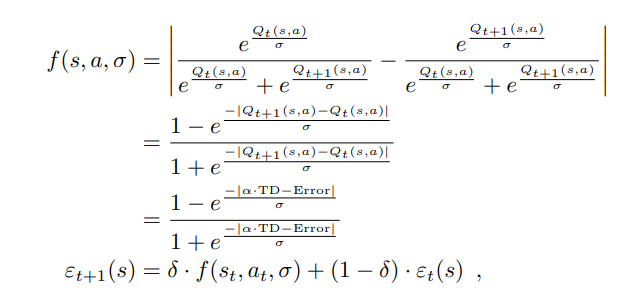
\includegraphics[width=0.8\linewidth]{VDBE_epsilon.png}
            \caption{\label{fig:VDBE_epsilon} На $s$ можно не обращать внимания, $a$ -- выбранное на $t$-ом шаге действие, $\sigma$ -- температура: чем выше, тем ближе распределение к равномерному, чем меньше, тем ближе к жадному \cite{tolic_VDBE}}
        \end{figure}
        \item Epsilon-BMC. Пока не разобрался.
    \end{enumerate}
    В \href{https://en.wikipedia.org/wiki/Multi-armed_bandit}{Википедии} также описаны эти стратегии
    \item Если знаем, какому семейству распределений принадлежат рычаги, то можно для матожиданий и дисперсии в первых двух алгоритмах использовать границы (например) $95\%$-го доверительного интервала.
\end{enumerate}

\subsection{Optimistic initialization}
Можно инициализировать начальные значения всех рычагов большим положительным числом, как и в обычной оптимистичной инициализации. Изменять матожидание можно как среднее арифметическое, так и скользящим окном: $Q_{t+1}(a) = Q_t(a) + \alpha (R_t - Q_t(a))$.

Аналогично с $\overline{R_{t+1}^2(a)}$: $\overline{R_{t+1}^2(a)} = \overline{R_{t}^2(a)} + \alpha (R_t^2 - \overline{R_{t}^2(a)})$.

Выборочная дисперсия изменяется по формуле \ref{eq:1}. Но думаю, что оптимистичная инициализация с const step-size будет работать плохо, как и в обычной задаче о многоруких бандитах.

\subsection{UCB}
Можно ввести UCB для приближения, которое строится, исходя из выбранных ранее рычагов (\ref{subsec:1}). То есть, аналогично классическому UCB, $A_t = \underset{a}{\arg \max} \left( Q_t(a) - 2 \lambda p_a S_t^2(a) + c \sqrt{\frac{\ln t}{N_t(a)}} \right)$, где $p_a = \frac{N_t(a)}{t-1}$.

Можно еще пытаться что-то проделать с софтмаксом ($H_t(a)$ зависит от $Q_t(a), \, S_t^2(a), \, t, \, N_t(a)$, и $p_a = \frac{e^{H_t(a)}}{\sum_{i=1}^n e^{H_t(i)}}$). Но вот здесь уже меньше уверенности, что сработает.

\subsection{Gradient bandits}

Проводя аналогичные вычисления, что и в параграфе из книги ``Reinforcement Learning: An Inrtroduction'' \cite{suttonbarto_gradient_bandits}, получаем:
\[
    H_{t+1}(a) = H_t(a) + \alpha \frac{\partial \mathbb{E}(Q_{t,p} - \lambda S_{t,p}^2)}{\partial H_t(a)}
\]
\begin{dmath}
    \frac{\partial \mathbb{E}(m_{\pi} - \lambda \sigma_{\pi}^2)}{\partial H_t(a)} = \sum_{x} \left( m_x - 2 \lambda \pi_t(x) \sigma_x^2 \right) \frac{\partial \pi_t(x)}{\partial H_t(a)} = \mathbb{E} \left( \frac{m_{A_t}}{\pi_t(A_t)} - 2 \lambda \sigma_{A_t}^2 - B_t \right) \frac{\partial \pi_t(A_t)}{\partial H_t(a)} = \mathbb{E} \left( m_{A_t} - 2 \lambda \pi_t(A_t) \sigma_{A_t}^2 - B_t \right) \left( \mathbb{I}_{a=A_t} - \pi_t(a) \right) = \mathbb{E} \left( R_t  - 2 \lambda \pi_t(A_t) S_{t+1}^2 (A_t) - B_t \right) \left( \mathbb{I}_{a=A_t} - \pi_t(a) \right) = \mathbb{E} \left( R_t  - 2 \lambda \pi_t(A_t) \frac{N_t(A_t) \overline{R_t^2(A_t)} - 2Q_t(A_t)R_t + R_t^2}{N_t(A_t) + 1} - B_t \right) \left( \mathbb{I}_{a=A_t} - \pi_t(a) \right)
\end{dmath}
Осталось выбрать baseline. Пусть $\overline{R_t^k} = \frac{\sum_{i=1}^{t-1} R_i^k}{t - 1}$, тогда возьмем
\[
\text{baseline} = \overline{R_t} - 2 \lambda \pi_t(A_t) \frac{N_t(A_t) \overline{R_t^2(A_t)} - 2Q_t(A_t) \overline{R_t} + \overline{R_t^2}}{N_t(A_t) + 1}
\]
так как $\forall k \; \mathbb{E} R_k^i = \mathbb{E} R_t^i$.
Итоговая формула:
\begin{dmath}
    H_{t+1}(a) = H_t(a) + \alpha \left[ R_t  - 2 \lambda \pi_t(A_t) \frac{N_t(A_t) \overline{R_t^2(A_t)} - 2Q_t(A_t)R_t + R_t^2}{N_t(A_t) + 1} - \overline{R_t} + 2 \lambda \pi_t(A_t) \frac{N_t(A_t) \overline{R_t^2(A_t)} - 2Q_t(A_t) \overline{R_t} + \overline{R_t^2}}{N_t(A_t) + 1} \right] \left( \mathbb{I}_{a=A_t} - \pi_t(a) \right) = H_t(a) + \alpha \left[ \left(1 - \frac{4 \lambda \pi_t(A_t) Q_t(A_t)}{N_t(A_t) + 1}\right) (R_t - \overline{R_t}) + \frac{2 \lambda \pi_t(A_t)}{N_t(A_t) + 1} (R_t^2 - \overline{R_t^2})\right] \left( \mathbb{I}_{a=A_t} - \pi_t(a) \right)
\end{dmath}
Подсчет суммарно всех $H_{t+1}(a)$ происходит за $O(1)$, если знаем $Q_t(A_t)$ и $N_t(A_t)$.

\subsection{Сэмплирование Томпсона}

Если нам известно, из какого семейства распределений взяты распределения для рычагов (например, из распределения Стьюдента с 3 степенями свободы), то в некоторых случаях можно найти сопряженное семейство распределений. Тогда для обычной задачи о многоруких бандитах можно использовать алгоритм, известный как сэмплирование Томпсона \cite{intro_bandits}: можно считать, что параметры исходного семейства распределений были взяты, исходя из сопряженного семейства распределений. В таком случае, хоть нам и неизвестны исходные параметры, но мы можем оценить их апостериорную вероятность. Исходный алгоритм выглядит так:
\begin{enumerate}
    \item Для каждого рычага сэмплируются матожидания в соответствии своим апостериорным вероятностям
    \item Выбирается рычаг с максимальным сэмплированным матожиданием
    \item Для выбранного рычага выдается награда и обновляются параметры для распределения из сопряженного семейства распределений, соответствующего этому рычагу. Тем самым изменяется представление о том, чему равно матожидание для выбранного рычага.
    \item Возврат к шагу 1.
\end{enumerate}
Сэмплирование Томпсона обладает весомым достоинством -- оно очень быстро находит рычаг с наибольшим матожиданием. А именно: матожидание сожаления $\mathbb{E} \: \overline{\text{Regret}_T} = O\left(\sqrt{n \frac{\log T}{T}} \right)$. Это значительный результат, поскольку, например, для любой стратегии с неадаптивным (то есть не зависящим от истории наград) исследованием при фиксированных $T, n$ существуют распределения на рычагах, при которых  $\mathbb{E} \: \overline{\text{Regret}_T} \geq \Omega \left(n^{1/3} \, T^{-1/3} \right)$ \cite{intro_bandits_slow_convergence}.

Сэмплирование Томпосна можно обобщить для случаев, когда выбор рычага не детерминирован. Рассмотрим такую модификацию для нашей задачи:
\begin{enumerate}
    \item Для каждого рычага сэмплируются матожидания и дисперсии в соответствии своим апостериорным вероятностям
    \item С помощью градиентного подъема или алгоритма за $O(n \log n)$ для выбранных матожиданий и дисперсий находится $P^* = \underset{P \in Q}{\arg \max} (m_P - \lambda \sigma_P^2)$
    \item Выбирается рычаг в соответствии с $P^*$.
    \item Для выбранного рычага выдается награда и обновляются параметры для распределения из сопряженного семейства распределений, соответствующего этому рычагу. Тем самым изменяется представление о том, чему равны матожидание и дсиперсия для выбранного рычага.
    \item Возврат к шагу 1.
\end{enumerate}

Возможно, это не будет работать, но попробовать стоит.

\section{Гитхаб}

 Статью также можно найти \href{https://github.com/davynchi/diploma/blob/main}{в этом репозитории} в папке "theoretical notes".

\bibliographystyle{alpha}
\bibliography{theory.bib}

\end{document}